\begin{refsection}

\chapter{Fission tracks}\label{ch:FT-R}

\noindent\begin{minipage}[t]{.25\linewidth}
\strut\vspace*{-\baselineskip}\newline
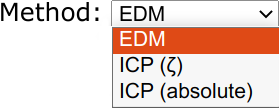
\includegraphics[width=\linewidth]{../figures/FTformats.png}
\end{minipage}
\begin{minipage}[t]{.75\linewidth}
  \texttt{IsoplotR} accepts three types of fission track data, as
  described in Chapter~\ref{ch:fissiontracks}.
\end{minipage}

\begin{enumerate}

\item\noindent\begin{minipage}[t]{.60\linewidth}
\strut\vspace*{-\baselineskip}\newline
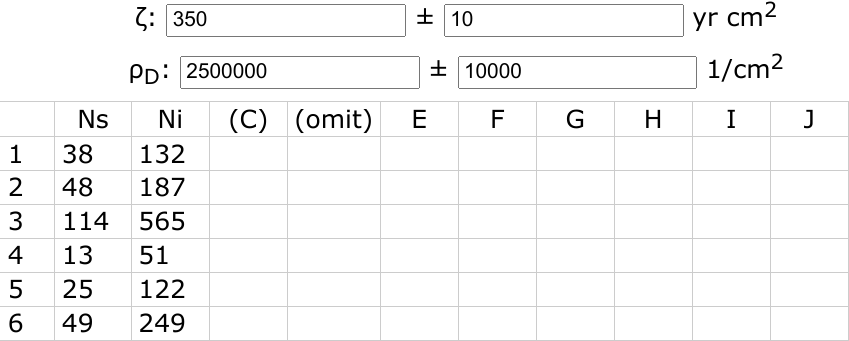
\includegraphics[width=\linewidth]{../figures/FTEDM.png}
\end{minipage}
\begin{minipage}[t]{.40\linewidth}
  The External Detector Method (EDM) requires the
  \textzeta-calibration factor and dosimeter glass track density
  ($\rho_D$) and standard errors, as well as a table with spontaneous
  and induced fission track counts. It is assumed that these were
  counted over the same area.
\end{minipage}

\begin{console}
FT1 <- read.data('FT1.csv',method='fissiontracks',format=1)
\end{console}

\noindent which returns a list with four items:

\begin{enumerate}
\item\texttt{format} stores the value of the eponymous argument,
\item\texttt{zeta} is a two-element vector with the
  \textzeta-calibration factor and its standard error,
\item\texttt{rhoD} is a two-element vector with the dosimeter glass
  density and its standard error,
\item\texttt{x} is a 2-column matrix with the fission track counts.
\end{enumerate}

\item LA-ICP-MS based fission track dating is implemented in two
  forms.  The first of these is \textzeta-calibration approach that is
  similar to the EDM. This approach does not require that the
  U-concentration estimates are 100\% accurate. It suffices that they
  are proportional to the actual U-concentrations. In fact, instead of
  specifying the U-concentrations, the \textzeta-calibration approach
  also accepts U/Ca-ratios, provided that the \textzeta-calibration
  constant has been obtained on a similar dataset.  Instead of a
  dosimeter glass density, the ICP-MS based approach requires that the
  user specify the spot size of the laser that was used to extract the
  U, Th (and Sm) from the sample.

\noindent\begin{minipage}[t]{.60\linewidth}
\strut\vspace*{-\baselineskip}\newline
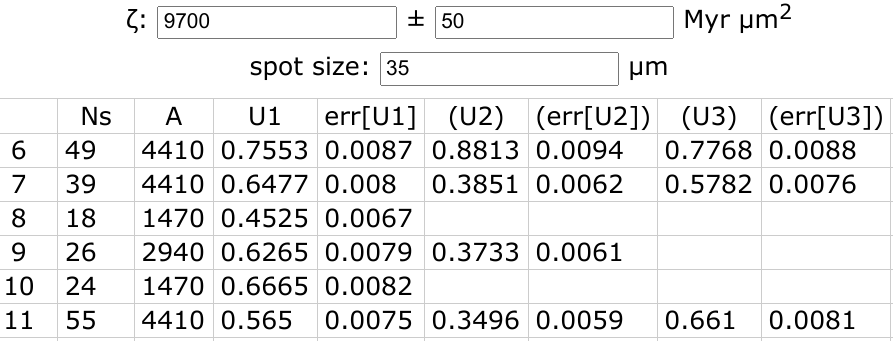
\includegraphics[width=\linewidth]{../figures/FTICPzeta.png}
\end{minipage}
\begin{minipage}[t]{.40\linewidth}
   The data table may contain a variable number of columns, reflecting
   the variable number of laser spots that may be placed in each grain
   in order to estimate the heterogeneity of the U-concentrations. The
   spot size is only used if at least one of the grains contains more
   than one U measurement.
\end{minipage}

\begin{console}
FT2 <- read.data('FT2.csv',method='fissiontracks',format=2)
\end{console}

\noindent which returns a list with seven items:

\begin{enumerate}
\item\texttt{format} stores the value of the eponymous argument,
\item\texttt{zeta} is a two-element vector with the
  \textzeta-calibration factor and its standard error,
\item\texttt{spotSize} is a scalar with the spot size of the laser
  ablation system,
\item\texttt{Ns} is a vector of spontaneous fission track counts.
\item\texttt{A} is a vector with the area (in
  \textmu{m}\textsuperscript{2}) over which the spontaneous tracks are
  counted.
\item\texttt{U} is a list of vectors, the list has the same length as
  \texttt{Ns} and \texttt{A}, and the vectors contain the
  U-concentration measurements of all the spots for each grain.
\item\label{it:ICPsU}\texttt{sU} is a second list of vectors that has
  exactly the same size as \texttt{U} but contains the standard errors
  of the U-concentration measurements.
\end{enumerate}

\item A second approach to ICP-based fission track dating is to trust
  the accuracy of the U-concentration measurements and use
  Equation~\ref{eq:tICP} to calculate the absolute age of each grain.

\noindent\begin{minipage}[t]{.60\linewidth}
\strut\vspace*{-\baselineskip}\newline
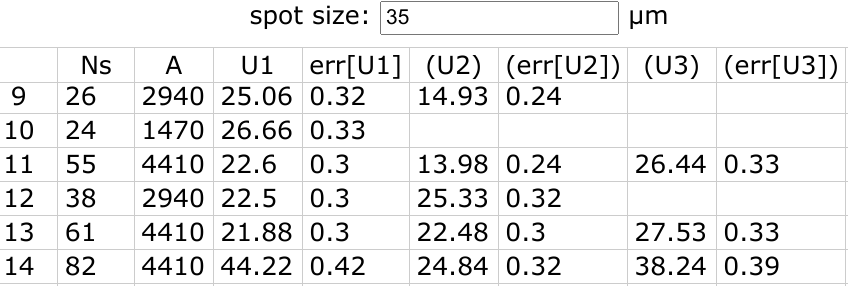
\includegraphics[width=\linewidth]{../figures/FTICPabsolute.png}
\end{minipage}
\begin{minipage}[t]{.40\linewidth}
  The input table of the absolute dating method looks identical to
  that of the \textzeta-calibration method. But in contrast with the
  latter method, the units of the U-concentration measurements must be
  ppm and U/Ca-ratios are not acceptable.
\end{minipage}

\begin{console}
FT3 <- read.data('FT3.csv',method='fissiontracks',format=3)
\end{console}

\noindent which returns a list with seven items:

\begin{enumerate}[leftmargin=\parindent,align=left]
\item[(a)~~]\texttt{format} stores the value of the eponymous argument,
\item[(b)~~]\texttt{mineral} is a text string that either equals
  \texttt{apatite} or \texttt{zircon},
\item[(c-g)]\texttt{spotSize}, \texttt{Ns}, \texttt{A},
  \texttt{U} and \texttt{sU} have the same meaning as for format 2.
\end{enumerate}

In contrast with the EDM and \textzeta-based ICP-MS dating, the
absolute dating method involves a host of other variables, which are
usually folded into the \textzeta-calibration factor. The default
\textsuperscript{238}U/\textsuperscript{235}U ratio is given by
\citet{hiess2012}, and the \textsuperscript{238}U decay constant by
\citet{jaffey1971}. The default value for the fission decay constant
is the consensus value of \citet{holden2000}.  The efficiency factor
($q$ in Equation~\ref{eq:tICP}) corrects the bias caused by the
etching process. The initial track length (or etchable range, $R_e$ in
Equation~\ref{eq:tICP}) is needed to convert the surface density
(tracks per unit area) into a volume density (tracks per unit
volume). Finally, the mineral density is needed to convert the uranium
concentration from ppm to atoms per unit volume.

\begin{center}
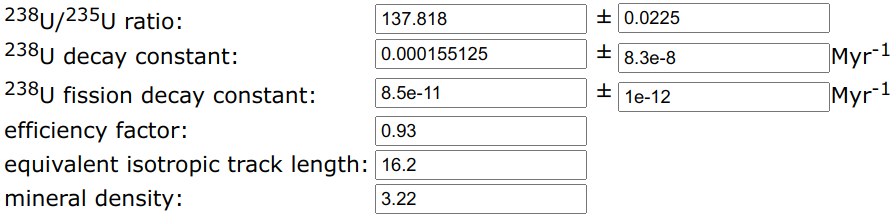
\includegraphics[width=.8\linewidth]{../figures/FTlambda.png}
\end{center}

The default efficiency factor for apatite is based on the mean of 3
measurements by \citet{iwano1998} and 1 measurement by
\citet{jonckheere2003b}. The default track length and mineral density
are nominal values that are commonly used in the literature.

\noindent\begin{minipage}[t]{.20\linewidth}
\strut\vspace*{-\baselineskip}\newline
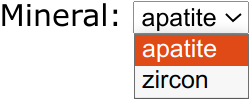
\includegraphics[width=\linewidth]{../figures/FTmineral.png}
\end{minipage}
\begin{minipage}[t]{.80\linewidth}
  The etch efficiency, initial track length and mineral density differ
  for zircon and apatite. \texttt{IsoplotR} includes appropriate
  presets for both of these minerals, which can be changed to any
  other value.
\end{minipage}

\begin{script}
# store the default density of zircon in a variable:
dens <- settings('mindens','zircon') 
# change the density setting for apatite:
settings('mindens','apatite',3.23)
# change the etch efficience factor for zircon:
settings('etchfact','zircon',0.99)
# change the etchable range for apatite to 15 microns:
settings('tracklength','apatite',15)
\end{script}

\end{enumerate}

\section{Radial plots}\label{FT-radial-R}

Radial plots were originally created for the purpose of visualising
fission track data, and are therefore ideally suited for this purpose.
For the external detector method, the radial plot is based on the raw
fission track counts:\\

\noindent\begin{minipage}[t]{.3\linewidth}
\strut\vspace*{-\baselineskip}\newline
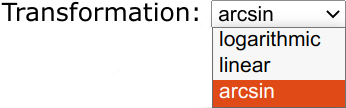
\includegraphics[width=\linewidth]{../figures/FTradialTransformations.png}
\end{minipage}
\begin{minipage}[t]{.7\linewidth}
  Like the generic radial plot of Section~\ref{sec:OtherRadial} and
  subsequent chapters, EDM-based radial plots can also be subjected to
  three transformations. But instead of a square root transformation,
  it implements an arcsine transformation (Equation~\ref{eq:zj}) as an
  optimal way to deal with zero data.
\end{minipage}

\begin{console}
radialplot(FT1,transformation='arcsin')
\end{console}

\noindent\begin{minipage}[t]{.3\linewidth}
\strut\vspace*{-\baselineskip}\newline
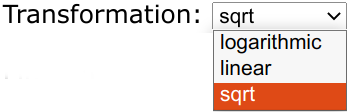
\includegraphics[width=\linewidth]{../figures/UPbRadialTransformation.png}
\end{minipage}
\begin{minipage}[t]{.7\linewidth}
For ICP-MS based fission track data, radial plots are generated from
the single grain ages rather than the raw fission track counts. So the
arcsin transformation is replaced by the square root transformation
again.
\end{minipage}

\begin{console}
radialplot(FT2,transformation='sqrt')
\end{console}

\noindent\begin{minipage}[t]{.4\linewidth}
\strut\vspace*{-\baselineskip}\newline

\includegraphics[width=\linewidth]{../figures/ArArExterr.png}
\end{minipage}
\begin{minipage}[t]{.6\linewidth}
  Ticking this box propagates the \textzeta-calibration and
  \textrho\textsubscript{D} uncertainty into the central age
  uncertainty.
\end{minipage}

\begin{console}
radialplot(FT2,exterr=TRUE)
\end{console}

\noindent\begin{minipage}[t]{.3\linewidth}
\strut\vspace*{-\baselineskip}\newline
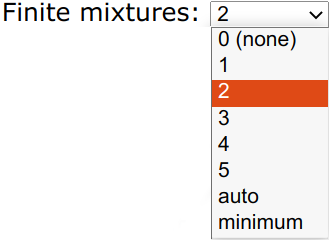
\includegraphics[width=\linewidth]{../figures/FTmixtures.png}
\end{minipage}
\begin{minipage}[t]{.7\linewidth}
  The mixture models for the EDM method use a different algorithm than
  those for the ICP-MS based data. However this complexity is hidden
  from the user and the interface remains exactly the same for both
  types of measurements.
\end{minipage}

\begin{console}
radialplot(FT1,k=2)
\end{console}

\section{\textzeta-calibration}

\texttt{IsoplotR} does not only use the \textzeta-calibration factor
to compute EDM or ICP-MS based fission track ages, but also provides
functionality to estimate the calibration factor.\\

\noindent\begin{minipage}[t]{.1\linewidth}
\strut\vspace*{-\baselineskip}\newline

\includegraphics[width=\linewidth]{../figures/RUN.png}
\end{minipage}
\begin{minipage}[t]{.9\linewidth}
  When `get \textzeta' is selected from the pull-down menu, the
  \texttt{PLOT} button changes to a \texttt{RUN} button.\\
\end{minipage}

The input data now contain the fission track counts (and
U-measurements) of an age standard. These follow the same format as
before, apart from the fact that the \textzeta-calibration box is
replaced by the age of the standard.\\

\noindent\begin{minipage}[t]{.5\linewidth}
\strut\vspace*{-\baselineskip}\newline
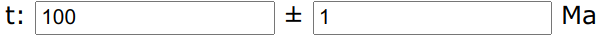
\includegraphics[width=\linewidth]{../figures/FTzetaT.png}
\end{minipage}
\begin{minipage}[t]{.5\linewidth}
Enter the age of the standard and its standard error, both in Ma.\\
\end{minipage}

Suppose that we use \texttt{FT1} to compute a zeta calibration factor
and its standard error:

\begin{console}
z <- set.zeta(x=FT1,tst=c(100,1))
\end{console}

\noindent\begin{minipage}[t]{.2\linewidth}
\strut\vspace*{-\baselineskip}\newline
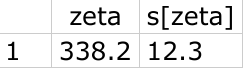
\includegraphics[width=\linewidth]{../figures/zetaoutput.png}
\end{minipage}
\begin{minipage}[t]{.8\linewidth}
The output of the function is not reported as a plot but as a small table.
\end{minipage}

\section{Age, weighted mean, KDE and CAD functions}

\begin{enumerate}

\item Like U--Th--He ages, also fission track data can be reliably (if
  imprecisely) determined on single crystals, without concerns about
  inherited daughter components.\\

\noindent\begin{minipage}[t]{.4\linewidth}
\strut\vspace*{-\baselineskip}\newline
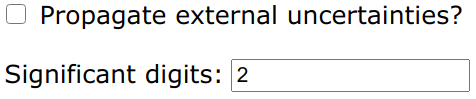
\includegraphics[width=\linewidth]{../figures/FTageSettings.png}
\end{minipage}
\begin{minipage}[t]{.6\linewidth}
It is normally best not to propagate the \textzeta-calibration
uncertainty into the single grain age uncertainty if the resulting
ages are to be jointly considered in subsequent data processing steps.
\end{minipage}

\begin{console}
age(FT1,exterr=FALSE)
\end{console}

\item The weighted mean age is less useful than the central age due to
  the heteroscedasticity of fission track data, but is provided
  nonetheless for the sake of completeness.

\begin{console}
weightedmean(FT3)
\end{console}

\item Similarly, KDEs are less informative for fission track data than the
  radial plot due to the large and variable measurement uncertainties.

\noindent\begin{minipage}[t]{.2\linewidth}
\strut\vspace*{-\baselineskip}\newline

\includegraphics[width=\linewidth]{../figures/UPbKDElogarithm.png}
\end{minipage}
\begin{minipage}[t]{.8\linewidth}
  However, when a KDE is used, then it is advisable to use a
  logarithmic transformation to account for the skewness of the
  counting uncertainties.
\end{minipage}

\begin{console}
kde(FT2,log=TRUE)
\end{console}

\item Like KDEs, also CADs do not explicitly account for the
  heteroscedasticity of fission track data. They tend to have a steep
  slope at the young end of the spectrum and gently level off towards
  old ages.

\begin{console}
cad(FT1)
\end{console}
  
\end{enumerate}

\printbibliography[heading=subbibliography]

\end{refsection}
